So far, we have only considered methods to sample static averages, which concern quantities at thermodynamic equilibrium.
Such techniques yield information about the bulk macroscopic properties of the system, for which there is no discernable macroscopic evolution.
We now turn to the next natural question, which is to consider systems in which there is such an evolution,
 which typically arises from a perturbation of the equilibrium dynamics, either by the introduction of a non-gradient forcing term, 
 or a modification of the fluctuation-dissipation part for which the fluctuation-dissipation relation \eqref{eq:general_fd_relation} is not verified.
 We will not consider the latter case, which is relevant for instance to the modelling of heat transport within an atomic system, to concentrate on the first case.
 In general, systems undergoing such a perturbation of the dynamics will reach a new steady state in which there is a net flux in some observable.
 Mathematically, this translate into the existence of a response observable $R$ which has zero average with respect to the canonical measure $\mu$, but which has a positive average with respect to the perturbation steady-state.
 A natural question is that of the sensitivity of the system to the perturbation: one way to quantify this is to modulate the strength of the perturbation by a positive real parameter $\eta>0$, and,
  assuming that the average response is asymptotically linear as $\eta\to 0$, to compute the linear coefficient linking $\eta$ and the average response. 
  This quantity is called a \textit{transport coefficient}, and we will dedicate the next two chapters to different methods of computing them using molecular simulation.

\section{Non-equilibrium molecular dynamics}
\subsection{General framework}
We first consider the most natural method, which is to directly apply a forcing term which is not the gradient of a periodic function. 
The general framework is that of a classical Langevin dynamics

\begin{equation}
    \label{eq:general_nemd_dynamics}
    \left\{\begin{aligned}
        \text dq_t&=M^{-1}p_t\dt,\\
        \text dp_t&= -\nabla V(q_t)\dt -\gamma M^{-1}p_t\dt+\sqrt{\frac{2\gamma}\beta}\text dW_t +\eta F(q_t)\dif t,
    \end{aligned}\right.
\end{equation}
perturbed by the configuration-dependent forcing term $F$, and where the strength of the perturbation is modulated by the parameter $\eta>0$.
Its generator is given by the operator 
\begin{equation}
    \label{eq:nemd_generator}
    \cL_{\gamma,F}=\cL_\gamma +\eta F\cdot \nabla_p = \cL_\gamma +\eta \widetilde{\cL}.
\end{equation}
It is also possible to consider non-equilibrium generalized Langevin equations, which are analogous perturbations of \eqref{eq:general_langevin}.
Given a response of interest $R$, the transport coefficient is given by the following definition:

\begin{equation}
    \label{eq:transport_coefficient}
    \rho_{R,F}=\underset{\eta \to 0}{\lim}\, \frac{\mathbb{E}[R]}{\eta},
\end{equation}
where $\mathbb{E}_\eta$ denotes the expectation with respect to the steady-state probability distribution. 
If the context makes $R$ clear from the knowledge of $F$, we will drop it from the notation and simply write $\rho_F$ for the transport coefficient.
For this definition to make sense, one has to show that the steady-state with respect to which we take the expectation is well-defined.
Since the steady-state is defined by the fact that it is invariant with respect to the dynamics \eqref{eq:general_nemd_dynamics}, 
this translate into the fact that it is the solution to a stationary Fokker-Planck equation, in the sense of distributions:
\begin{equation}
    \label{eq:nemd_fp_equation}
    (\cL_\gamma +\eta \widetilde{\cL})^\dagger \psi_\eta = 0,
\end{equation}
where $\psi_\eta$ is the steady state measure. Using analytic properties of $\cL_{\gamma,F}$ (such as hypoellipticity), one can hope to infer regularity results of its solutions, such as the existence of a smooth density.
Existence and unicity can in principle be inferred following Klieman's method \cite{K87}. 
The steady-state measure $\E_\eta$ is a high-dimensional measure on phase space for which a closed form is generally unavailable.
 Thus, as usual, one has to resort to ergodic averages under the dynamics \eqref{eq:general_nemd_dynamics} to compute ensemble averages.
 This poses another theoretical difficulty, that of showing that the steady-state measure is ergodic.

In fact, for our purposes, $F$ will always be $L\mathbb{T}^{dN}$-periodic, and so we can invoke a special case of Proposition 1 in \cite{JPS15} with time-constant forcings, provided $V$ and $F$ are smooth.
\begin{theorem}[Existence of a unique ergodic measure with smooth density]\label{thm:nemd_exst_invariant_measure}
    Let $\eta_*>0$. For all $\eta\in[-\eta_*,\eta_*]$, the Fokker-Planck equation \eqref{eq:nemd_fp_equation} admits a unique solution with a $C^\infty$ density $\psi_\eta$.
    Additionally, the evolution semi-group decays exponentially in a Lyapunov sense: for all $n\geq 1$, there exist $C_n,\,\lambda_n>0$ such that
    \begin{equation}
        \label{eq:lyapunov_exp_decay}
        \left\|\e^{t\cL_{\gamma,F}}\varphi-\E_\eta[\varphi]\right\|_{L^{\infty}(\mathcal E)}\leq C_n\e^{-\lambda_n t}\|\varphi\|_{L^\infty_{\mathcal K_n}},
    \end{equation}
    where we define the Lyapunov weight functions
    \[\mathcal K_n(q,p)=1+|p|^{2n},\]
    and the corresponding weighted $L^{\infty}$ spaces by the norm
    \[\|f\|_{L^\infty_{\mathcal K_n}}=\left\|\frac{f}{\mathcal K_n}\right\|_{L^\infty(\mathcal E)}.\]
\end{theorem}
Because of the continuous injections $L^\infty \subset L^\infty_{\mathcal K_n}$, this result implies in particular that the operator 
$(-\cL_{\gamma,F})^{-1}$ is well-defined on 
\[L^\infty_{\mathcal K_n,0}=\left\{f\in L^\infty_{\mathcal K_n}\middle|\,\E_\eta[f]=0\right\},\]
with an inverse given by the formula \eqref{eq:resolvent_langevin}. Proposition 2 from the same papers also gives the almost-sure convergence of ergodic averages.
 \begin{remark}[Size of the linear regime]
    As $\eta \to 0$, it is reasonable to expect that the statistical error in ergodic averages for
    $\E_\eta[R]$ arise at dominant order in $\eta$ from the asymptotic variance at equilibrium $\sigma^2_R$ \eqref{eq:asymptotic_variance_with_Lm1}.
    In particular the finite difference estimator for $\rho_{R,F}$
    \begin{equation}
        \label{eq:fd_estimator_rho_F}
        \frac{\mathbb{E}_\eta[R]}{\eta}
    \end{equation}
    has, for a fixed simulation time, a variance which scales like $\frac1{\eta^2}$ as $\eta\to 0$.
    To achieve an acceptable statistical error at minimal cost, one should thus aim to take $\eta$ as large as possible.
    On the other hand, if the perturbation is too large, then non-linear effects on $R$ will be observed and \eqref{eq:fd_estimator_rho_F} 
    will give a poor estimation of the transport coefficient.
    Thus, if one manages to devise another forcing $\tilde F$ which does not change the steady-state, but which extends the range of linearity of the response,
    it may be very benificial to do so from a computational standpoint. These kinds of methods, sometimes called synthetic forcings, are an area of ongoing research. (ref...)
 \end{remark}
\subsection{Numerical implementation}
To integrate the perturbed dynamics, we again rely on a splitting strategy.
We split the dynamics into elementary evolutions, whose respective evolution semigroups are given analogously to \eqref{eq:propagators}.
The only difference is in the additional $\eta F$ term, which we incorporate into the $B$ step, yielding a $B_{\eta F}$ step, which corresponds to the evolution semi-group
\begin{equation}
    \label{eq:B_etaF_step}
    \e^{tB_{\eta F}}\varphi(q,p)=\varphi(q,p-t\left(\nabla V(q)-\eta F(q)\right)).
\end{equation}
Note it would also have been possible to incorporate the forcing term into the Ornstein-Uhlenbeck part of the dynamics, which then corresponds to an Ornstein-Uhlenbeck process with constant drift.
However, we will always choose the method described above. We will use the same terminology for these methods, referring to the scheme with evolution operator
\begin{equation}
    \e^{\frac{\Dt}2B_{\eta F}}\e^{\frac{\Dt}A}\e^{\Dt\gamma C}\e^{\frac{\Dt}2A}\e^{\frac{\Dt}2B_{\eta F}}
\end{equation}
as the BAOAB scheme, for example.
Numerical estimates for $\E_\eta[R]$ are then obtained through 
\begin{equation}
    \label{eq:nemd_response_estimator}
    \widehat{R}_{\eta,N_{\mathrm{iter}}}= \frac{1}{N_{\mathrm{iter}}}\sum_{n=0}^{N_\mathrm{iter}-1} R(q^n,p^n),
\end{equation}
where $(q^n,p^n)_{n\geq 0}$ denote the numerical trajectory under the Markov chain obtained for a chosen splitting of the non-equilibrium dynamics \eqref{eq:general_nemd_dynamics}.
To estimate the transport coefficient, we fix different forcing intensities
\[0<\eta_1<\dotsm<\eta_k,\qquad \eta\defeq (\eta_i)_{1\leq i\leq k}\]
all in the linear response regime, and given corresponding estimators 
\[\widehat{R} \defeq (\widehat{R}_i)_{1\leq i\leq k}\]
of the form \eqref{eq:nemd_response_estimator}, we estimate $\rho_F$ by a least squares linear fit 
\begin{equation}
    \label{eq:rho_F_nemd_estimator}
    \widehat{\rho}_F= |\eta|^{-2}\eta\cdot\widehat{R}= \underset{\rho \in \R}{\mathrm{argmin}} \left| \rho\eta - \widehat{R}\right|^2.
\end{equation}
Note the case $k=1$ recuperates the finite difference estimator \eqref{eq:fd_estimator_rho_F}.
\subsection{Mobility}
As a first and simplest example, we introduce a method for computing the mobility. In this case the forcing is simply a constant vector, and the response is velocity in the direction $F$, which we may think of as the particle flux through $F$'s orthogonal hyperplane.
\begin{equation}
    \label{eq:nemd_mobility_definitions}
    F\in \R^{dN}\,\qquad R(q,p)=F\cdot M^{-1}p.
\end{equation}
Let us assume once and for all that $|F|^2=1$.
For practical computations, we will be considering two cases:
\begin{enumerate}[(i)]
    \item \textbf{Single drift}: this corresponds to a perturbation where the force acts on a single component of the momentum, which we can assume by indistinguishability of the particles to be the x component of the first particle, \[F=(1,0,\dots)^\intercal \in \R^{dN}.\]
    \item \textbf{Color drift}: this corresponds to a perturbation in which we the force acts on half of the particles in one direction, and on half of the particles in the opposite direction. By isotropy, we may assume this direction is the x direction, \[F=\frac1{\sqrt N}\underbrace{(1,0,\dots,}_{d \text{ components}}-1,0,\dots,1,0\dots)^\intercal \in \R^{dN}.\]
\end{enumerate}
The color drift method derive its name from the fact that it divides the particles into two categories: the particles with a positive color charge (corresponding to those whose x-component of momentum see a positive force contribution from $F$), and those with a negative color charge.
The equations of motion are analogous to a system of charged particles under a constant electric field, but where the charges do not interact between themselves.
The idea is taken from \cite{EM08}, Chapter 6. Intuitively, we expect the color drift method to be more economical than the single drift method, since the latter should give essentially equilibrium dynamics for the majority of particles outside of the first particle's sphere of influence.
On the other hand, the normalization condition implies that the forcing is more dilute in the color drift case, which may make the response more difficult to measure. In fact, numerical evidence presented below shows that the two effects roughly compensate one another.

In order for the two methods to be useful, we need to be able to relate them to a shared dynamical property of the considered system.
Doing is more conveniently done upon reformulating the linear response in terms of integrated autocorrelation functions, a point we postpone to the next section.
For now, let us show a few numerical results.
In order to compare different methods, we fix a thermodynamical condition, which we give in reduced units below.
\begin{equation}
    \label{eq:reference_thermo_condition}
    T=1.25,\quad \rho=0.6,\quad \gamma=1.0,\quad N=1000.
\end{equation}

Let us also mention here that all simulations for mobility were performed using a BAOAB splitting, a timestep $\Dt=10^{-3}$ and a linearly corrected cutoff at distance $r_c=2.5$.
In Figure \ref{fig:nemd_mobility_full}, we plot the response profile as a function of the forcing intensity. 
It appears that the linear response regime is longer for the color drift method.
Estimates of $\rho_F$ seem to roughly agree, although it is dubious that the small discrepancy observed is due to a systematic effect rather than statistical fluctuations persisting after very long integration times (all simulations for $\eta\leq 1$ ran for reduced physical times of over $2.5 \times 10^5$).
\begin{figure}[htbp]
    \begin{center}
      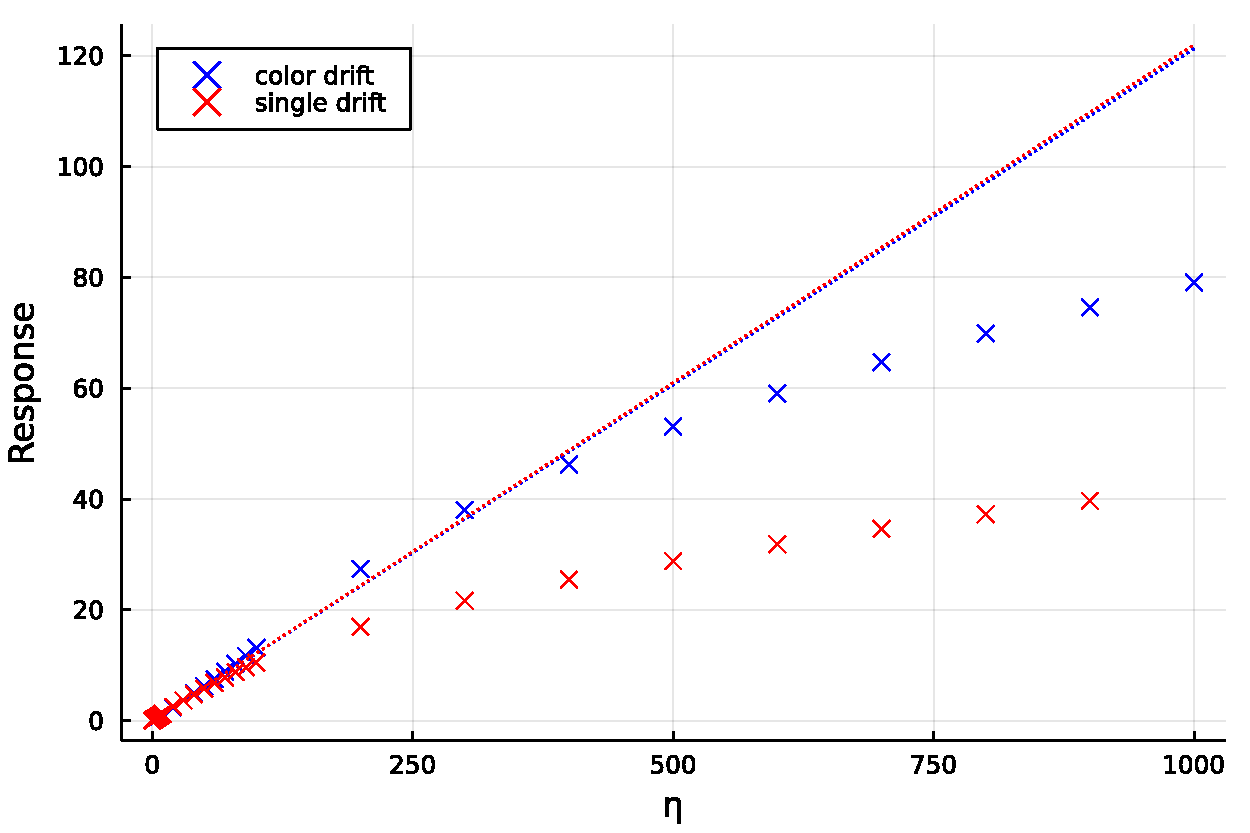
\includegraphics[width=0.7\linewidth]{figures/nemd/nemd_mobility_full.pdf}
      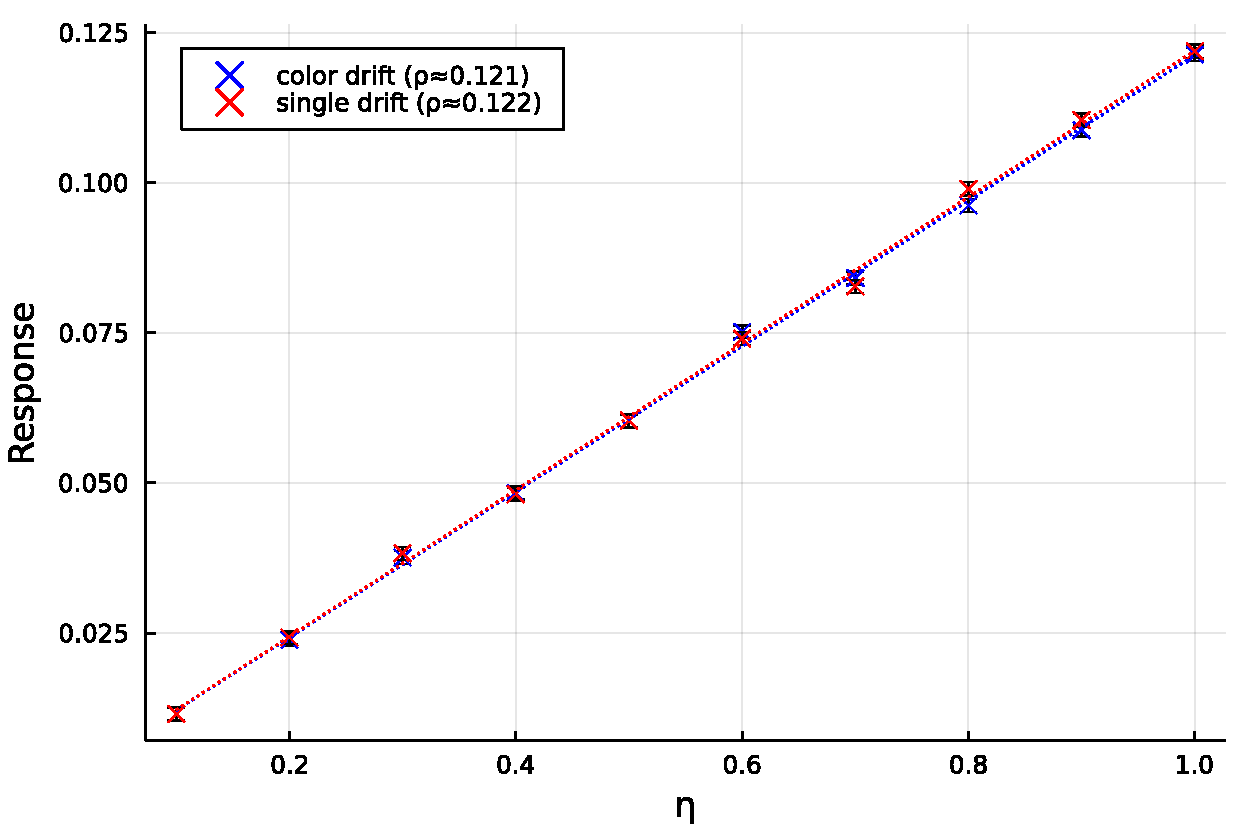
\includegraphics[width=0.7\linewidth]{figures/nemd/nemd_mobility_linear.pdf}
      \caption{ \label{fig:nemd_mobility_full}
        Average mobility response against forcing intensity for the Lennard-Jones system \eqref{eq:reference_thermo_condition}. Extrapolations of the linear response are plotted in dotted lines.
      }
    \end{center}
  \end{figure}
\subsection{Shear viscosity}
As a second example, we discuss the methods of \cite{JS12} for computing shear-viscosity. We refer to this paper for thorough statements and proofs.
Let us assume for notational simplicity that $M=m\Id$.
We consider a case of the dynamics \eqref{eq:general_nemd_dynamics} with a forcing which acts on the longitudinal (x) momenta, and is dependent on the transverse (y) positions.
More precisely, we fix a reference periodic function $F_y:L\mathbb{T}\longrightarrow \R$,
and index the state as \[\left(q_{i\alpha}\right)_{\substack{\leq i\leq N\\1\leq \alpha\leq d}},\qquad \left(p_{i\alpha}\right)_{\substack{\leq i\leq N\\1\leq \alpha\leq d}}.\]
The non-equilibrium dynamics is defined by the following expression for $F$:
\begin{equation}
    \label{eq:shear_viscosity_forcing}
    \forall\, 1\leq i\leq N,\,\forall\, 2\leq \alpha\leq d,\qquad F(q)_{i1}=F_y(q_{i2}),\qquad F(q)_{i\alpha}=0.
\end{equation}
The idea is that by imposing a forcing \textit{profile} in the x-direction, we observe a velocity profile in response, which depends on the $y$-coordinate.
\begin{remark}[Anisotropic friction]
    In fact the precise model considered in \cite{JS12} also imposes a separate friction coefficient $\gamma_x$ for the longitudinal fluctuation-dissipation part of the dynamics.
    This can be interpreted as a simple case of a generalized Langevin dynamics where the friction coefficient $\gamma$ is an anisotropic diagonal matrix, which does not pose any difficulties from the theoretical point of view.
    We therefore restrict our attention to the case where $\gamma$ is scalar.
\end{remark}
More precisely, we define
\begin{equation}
    \label{eq:velocity_profile}
    u_x(Y)\defeq \underset{\epsilon \to 0}{\lim} \, \underset{\eta \to 0}{\lim} \frac{L_y\E_\eta \left[\sum_{i=1}^N p_{i1}\chi_\epsilon(q_{i2}-Y)\right]}{\eta mN}
\end{equation}
to be the linear response profile in the longitudinal velocity, where $(\chi_\epsilon)_{\epsilon>0}$ is an approximation to the identity (that is a sequence of smooth compactly supported test functions which converge to the Dirac delta function in the sense of distributions).
In practice, $u_x$ can be estimated from numerical trajectories by decomposing the domain $\mathcal D$ in a finite number of transverse slices,
 and measuring the average longitudinal velocity in each of these slices.
 The shear viscosity $\sigma$ is then defined by the differential equation
\begin{equation}
    \label{eq:shear_viscosity_relation_diffeq}
    \sigma u_x''(Y)+\gamma \rho u_x(Y)=\rho F_y(Y),
\end{equation}
where $\rho= N/L^3$ is the particle density.
In fact, the solutions to \eqref{eq:shear_viscosity_relation_diffeq} are periodic, thus the magnitude of the linear response can be estimated through Fourier-like coefficients.
This has the advantage of giving an estimation of the linear response in the general framework defined above, and avoiding the discretization error arising from the finite number of transverse slices.
To this effect, we define the response observables as empirical Fourier coefficients (or imaginary parts thereof):
\begin{equation}
    \label{eq:nemd_shear_viscosity_response}
    R_k(q,p)=\frac{1}N\sum_{i=1}^N\frac{p_{i1}}{m}\sin\left(\frac{2k\pi q_{i2}}{L}\right).
\end{equation}
provided $F_y$ is not orthogonal to the family
\[\left\{ y\mapsto \sin\left(\frac{2k\pi y}{L}\right),\,k\geq 1\right\} ,\]
in $L^2([0,L))$, these observables give a meaningful measure of the linear response. In practice, it is sufficient to consider $k=1$ and carefully choose the forcing.
\begin{remark}
    To obtain better statistics, one may for the purpose of numerical simulations want to consider a periodic domain whose unit cell is still a cuboid, but with a side length in the longitudinal direction that is longer than in the transverse direction.
    In this case we simply replace $L$ by $L_y$ in the response observables, where $L_y$ is the length of the unit cell in the transverse direction.
\end{remark}
The shear viscosity can then be computed from equation \eqref{eq:shear_viscosity_relation_diffeq}, given an estimator $\widehat{R}_{k,N_{\mathrm{iter}}}$ of the form \eqref{eq:nemd_response_estimator}, through
\begin{equation}
    \label{eq:shear_viscosity_nemd_estimator}
    \hat{\sigma}_{N_{\mathrm{iter}}}=\rho\left(\frac{F_k}{\widehat{R}_{k,N_{\mathrm{iter}}}}-\gamma\right)\left(\frac{L}{2k\pi}\right)^2,
\end{equation}
again considering $k=1$ in practice.
\section{The Green-Kubo method}
An alternative route to the perturbation method described above leverages a famous expression for the transport coefficient in terms of an integrated correlation function, or, in less prosaic language, in terms of the fluctuations at equilibrium of the response observable.
This is the Green-Kubo method, which we describe in this section. We consider the invariant measure for the non-equilibrium dynamics \eqref{eq:general_nemd_dynamics}. By Theorem \ref{thm:nemd_exst_invariant_measure}, there exists a unique invariant measure with density $\psi_\eta$.
For notational consistency, let us write $\psi_0$ for the density of the equilibrium measure $\mu$. Then the following result holds 
\begin{theorem}[Series expansion for the non-equilibrium steady state]
    \label{thm:nemd_steady_state_series}
    There exists $r>0$ such that for all $0<\eta<r$,
    \begin{equation}
    \label{eq:nemd_steady_state_series}
        \frac{\psi_\eta}{\psi_0}=\left(1+\eta(\widetilde{\cL} \Pi \cL_\gamma^{-1}\Pi)^*\right)^{-1}\1_{\mathcal E}=\left(1+\sum_{k=1}^{\infty}(-\eta)^k\left[(\tilde \cL \Pi\cL_\gamma^{-1}\Pi)^*\right]^k\right)\1_{\mathcal E},
    \end{equation}
    where $\widetilde{\cL}$ is defined by \eqref{eq:nemd_generator}, $\Pi$ is the equilibrium centering projector defined in \eqref{eq:equilibrium_projector}, and the adjoint is taken in $L^2(\mu)$.
\end{theorem}
\begin{proof}[Sketch of proof]
    The second equality identifies the Neumann series on the right as the resolvent of $-(\widetilde{\cL} \Pi \cL_\gamma^{-1}\Pi)^*$, provided $\eta$ is taken small enough.
    In fact, from the spectral theory of bounded operators, $r$ can be determined as the spectral radius of $(\widetilde{\cL} \Pi \cL_\gamma^{-1}\Pi)^*$ in the space of bounded operators $\mathcal{B}(L^2_0(\mu))$.
    The core of the argument lies in making the ansatz
    \begin{equation}
        \label{eq:nemd_measure_ansatz}
        \psi_\eta=\psi_0(1+\eta f_1+\eta^2 f_2+\dotsm).
    \end{equation}
    The stationary Fokker-Planck equation \eqref{eq:nemd_fp_equation} writes
    \[(\cL_\gamma +\eta \widetilde{\cL})^{\dagger}\psi_0(1+\eta f_1+\eta^2 f_2+\dotsm)=(\cL_\gamma +\eta \widetilde{\cL})^{*}(1+\eta f_1+\eta^2 f_2+\dotsm)=0.\]
    By formally separating terms by degree in $\eta$, we obtain
    \begin{align*}
        \cL_\gamma^* \1_\mathcal E&=0,\\
        \widetilde{\cL}^*\1_{\mathcal E}+\cL_\gamma^*f_1&=0,\\
        \widetilde{\cL}^*f_1+\cL_\gamma^*f_2&=0,
    \end{align*}
    and so on. Note that the first equality is the equilibrium Fokker-Planck equation.
    Thus, by induction, again formally, we obtain.
    \begin{align*}
        f_1 &= (-\cL_\gamma^*)^{-1}\widetilde{\cL}^*\1_{\mathcal E},\\
        f_2 &= (-\cL_\gamma^*)^{-1}\widetilde{\cL}^*f_1,\\
        &\dotsm\\
        f_n &= \left[(-\cL_\gamma^*)^{-1}\widetilde{\cL}^*\right]^{n}\1_{\mathcal E},
    \end{align*}
    whence the formal proof follows, by observing that we can write 
    \[(-\cL_\gamma^*)^{-1}\widetilde{\cL}^*=-(\widetilde{\cL} \Pi \cL_\gamma^{-1}\Pi)^*.\]
    For a rigorous proof, several points should be made precise:
    \begin{enumerate}[(i)]
        \item The convergence of the series \eqref{eq:nemd_steady_state_series} for sufficiently small $\eta$, which can be obtained by showing the boundedness of the operator \[(\widetilde{\cL} \Pi \cL_\gamma^{-1}\Pi)^*\] on $L_0(\mu)$.
        \item The fact that \[\psi_0\left(1+\eta(\widetilde{\cL} \Pi \cL_\gamma^{-1}\Pi)^*\right)^{-1}\1_{\mathcal E}\] is indeed a solution to the stationary Fokker-Planck equation.
        \item The fact that it is indeed a probability density. 
    \end{enumerate}
    One can then conclude by unicity of the steady-state measure.
\end{proof}
Strikingly, we can read the linear response directly from the first term of the series expansion.
\begin{corollary}[Green-Kubo formula]
    Let $R$ be any response observable such that $\E_\mu[R]=0$, and $R\in L^{\infty}_{\mathcal{K}_n}$ for some $n$.
    Then we have the following formula for the linear response
    \begin{equation}
        \label{eq:green_kubo}
        \underset{\eta\to 0}{\lim}\,\frac{\E_{\eta}[R]}{\eta}=\int_0^\infty \E_\mu[R(q_t,p_t)S(q_0,p_0)]\dif t,
    \end{equation}
    where the expectation on the right hand side is with respect to all equilibrium dynamics trajectories with canonical initial distribution, and $S$ is defined by
    \begin{equation}
        \label{eq:conjugate_response}
        S=\widetilde{\cL}^*\1_{\mathcal E}=\beta F(q)\cdot M^{-1}p,
    \end{equation}
    and is called the conjugate response function. The latter expression follows from a simple integration by parts.
\end{corollary}
\begin{proof}
    By Theorem \ref{thm:nemd_steady_state_series}, we can write 
    \begin{align*}
        \underset{\eta\to 0}{\lim}\,\frac{\E_{\eta}[R]}{\eta}&=\int_{\mathcal E}R(q,p)(-\cL_\gamma^*)^{-1}\widetilde{\cL}^*\1_{\mathcal E}\psi_0(q,p)\,\dif q\, \dif p\\
        &=\int_{\mathcal E}(-\cL_\gamma)^{-1}R(q,p)S(q,p)\psi_0(q,p)\,\dif q\, \dif p\\
        &=\int_{\mathcal E}\int_0^\infty\E^{(q,p)}[R(q_t,p_t)S(q_0,p_0)]\psi_0(q,p)\,\dif t\,\dif q\,\dif p\\
        &=\int_0^\infty \E_\mu[R(q_t,p_t)S(q_0,p_0)]\,\dif t,
    \end{align*}
    where we rely on an expression like \eqref{eq:resolvent_langevin} for $(-\cL_\gamma)^{-1}.$
\end{proof}
The Green-Kubo formula has a great advantage, in that it allows us to estimate the transport coefficients for as many different perturbations and response observables as we want \textbf{from a single equilibrium trajectory}.
Indeed, one only needs to compute the corresponding integrated correlation functions \eqref{eq:green_kubo}.
\subsection{Numerical implementation}
We now describe a method to compute correlation functions necessary to the Green-Kubo method from a single long numerical trajectory.
This method is described by Tuckerman in \cite{T10}, section 13.4.2 for Hamiltonian trajectories.
In fact we consider a slight extension in which we let $R$ and $S$ to be vector-valued observables.
For notational simplicity, we assume that $R$ and $S$ are component-wise centered. The quantities we want to estimate are 
\begin{equation}
    \label{eq:time_correlation}
    C(t)=\E_\mu[R(q_t,p_t)^\intercal S(q_0,p_0)]
\end{equation}
we let $(q^n,p^n)_{n\geq 0}$ be a numerical trajectory, which we see as the random iterates of the Markov chain associated with a numerical scheme, with a regular timestep $\Dt>0$.
We further assume that the trajectory is stationary for this Markov chain, which is a realistic assumption if we take care of equilibriating the system using our numerical scheme before recording states.
By stationarity, the equality in law
\[(q^n,p^n,q^0,p^0) \overset{\mathrm{law}}{=}(q^{n+k},p^{n+k}q^k,p^k)\]
for all $k$. Hence we define the following estimator for $C(n\Dt)$, for $0\leq n\leq N_{\mathrm{iter}}:$
\begin{equation}
    \label{eq:ac_estimator}
    \widehat{C}_{N_{\mathrm{iter}}}(n\Dt) = \frac{1}{N_{\mathrm{iter}}-n+1}\sum_{k=0}^{N_{\mathrm{iter}}-n}R(q^{n+k},p^{n+k})^\intercal S(q^k,p^k).
\end{equation}
Note the quality of these estimators degrades with $n$. Thus in practice, we fix $N_{\mathrm{corr}}\ll N_{\mathrm{iter}}$, and compute these estimators for $0\leq n \leq N_{\mathrm{corr}}$.
For implementation details, we refer to the Appendix and links therein to relevant Julia code.

Using these estimators, we can estimate the transport coefficient through the Green-Kubo formula \eqref{eq:green_kubo}. The simplest way is to use a naive Riemann sum, or rectangle rule:
\[\rho_F \approx \Dt\sum_{k=0}^{N_{\mathrm{corr}}} \widehat{C}_{N_{\mathrm{iter}}}(k\Dt).\]
In fact, analysis shows that using a trapezoidal rule reduces the error.
However, these procedures introduce a truncation in time of the integral in \eqref{eq:green_kubo}.
Another approach consists of extrapolating the behavior of $\widehat{C}_{N_{\mathrm{iter}}}$ by fitting a parametric model 
\begin{equation}
    \label{eq:time_correlation_parametric_model}
    C_{\theta}(t)=\e^{-\lambda t}\left(\sum_{k=1}^{m}a_k\sin(f_k t+\omega_k)\right),
\end{equation}
where \[\theta=(\lambda,a_1,f_1,\omega_1,\dots,a_m,f_m,\omega_m)\in \R_{>0}\times\R^{3m}\]
is the parameter. The form of this model is justified empirically, although a formal argument based on a diagonalisation of the evolution semi-group can be made. 
Rigorously justifying and quantifying the accuracy of this model requires fine knowledge of the spectrum of $\cL_\gamma$.
At any rate, we can then fit the model in a least-squares sense,
\begin{equation}
    \theta^*=\underset{\theta\in \R_{>0}\times\R^{3m}}{\mathrm{argmin}}\sum_{n=0}^{N_{\mathrm{corr}}}\left| C_{\theta}(n\Dt)-\widehat{C}_{N_{\mathrm{iter}}}(n\Dt) \right|^2,
\end{equation}
for instance using gradient descent, and deduce the estimator for the transport coefficient,
\begin{equation}
    \label{eq:rho_F_estimator_GK_fit}
    \widehat{\rho}^{\mathrm{GK}}_{F,N_{\mathrm{iter}}}=\int_0^\infty C_{\theta^*}(t)\,\dif t,
\end{equation}
leveraging the elementary identity
\begin{equation}
    \label{eq:int_analytic_form}
    \int_0^{\infty}\e^{-\lambda t}a\sin(ft+\omega)\,\dif t=a\frac{\lambda\cos\omega-f\sin\omega}{f^2+\lambda^2}.
\end{equation}
\subsection{Mobility}
\subsection{Shear viscosity}